%% ============================================================
%%  Slides — Aproximaciones del kernel coseno
%%  Proyecto Clustering_Microbiota / Kernel_Tests
%%
%%  Compilar: pdflatex Slides_Cosine_Approx.tex (dos pasadas)
%%
%%  Imagenes esperadas (relativas a este .tex):
%%    report_assets/cosine_approx_error.png
%%    report_assets/cosine_approx_pareto.png
%%
%%  Si todavia no se ha corrido benchmark_cosine_approx.py, los
%%  \includegraphics fallan; comentar esos frames hasta tener los
%%  PNGs.
%% ============================================================
\documentclass[aspectratio=169,10pt]{beamer}

\usetheme{Madrid}
\usecolortheme{default}

%% Paleta (misma que Slides_Kernels_KDE_3.tex)
\definecolor{Navy}    {HTML}{1B2A4A}
\definecolor{Blue}    {HTML}{2563EB}
\definecolor{LBlue}   {HTML}{DBEAFE}
\definecolor{Teal}    {HTML}{0F766E}
\definecolor{LTeal}   {HTML}{CCFBF1}
\definecolor{Amber}   {HTML}{D97706}
\definecolor{LAmber}  {HTML}{FEF3C7}
\definecolor{Coral}   {HTML}{DC2626}
\definecolor{LCoral}  {HTML}{FEE2E2}
\definecolor{Green}   {HTML}{15803D}
\definecolor{LGreen}  {HTML}{DCFCE7}
\definecolor{Purple}  {HTML}{7C3AED}
\definecolor{LPurple} {HTML}{EDE9FE}
\definecolor{GrayMid} {HTML}{6B7280}
\definecolor{GrayLt}  {HTML}{F3F4F6}
\definecolor{GrayDark}{HTML}{374151}

\setbeamercolor{palette primary}   {bg=Navy,   fg=white}
\setbeamercolor{palette secondary} {bg=Blue,   fg=white}
\setbeamercolor{palette tertiary}  {bg=Teal,   fg=white}
\setbeamercolor{palette quaternary}{bg=Navy,   fg=white}
\setbeamercolor{structure}         {fg=Navy}
\setbeamercolor{frametitle}        {bg=Navy, fg=white}
\setbeamercolor{title}             {bg=Navy, fg=white}
\setbeamercolor{author in head/foot}{bg=Blue, fg=white}
\setbeamercolor{title in head/foot} {bg=Navy, fg=white}
\setbeamercolor{date in head/foot}  {bg=Teal, fg=white}
\setbeamercolor{block title}        {bg=Blue, fg=white}
\setbeamercolor{block body}         {bg=LBlue}
\setbeamercolor{block title alerted}{bg=Coral, fg=white}
\setbeamercolor{block body alerted} {bg=LCoral}
\setbeamercolor{block title example}{bg=Teal, fg=white}
\setbeamercolor{block body example} {bg=LTeal}

\usepackage[T1]{fontenc}
\usepackage[utf8]{inputenc}
\usepackage[spanish,es-tabla]{babel}
\usepackage{palatino}
\usepackage{microtype}
\usepackage{amsmath,amssymb}
\usepackage{graphicx}
\usepackage{booktabs}
\usepackage{array}
\usepackage{colortbl}
\usepackage{tikz}
\usepackage[most]{tcolorbox}

\setbeamertemplate{navigation symbols}{}

\setbeamertemplate{footline}{
  \leavevmode
  \hbox{
    \begin{beamercolorbox}[wd=.33\paperwidth,ht=2.25ex,dp=1ex,center]{author in head/foot}
      \usebeamerfont{author in head/foot}\insertshortauthor
    \end{beamercolorbox}
    \begin{beamercolorbox}[wd=.34\paperwidth,ht=2.25ex,dp=1ex,center]{title in head/foot}
      \usebeamerfont{title in head/foot}\insertshorttitle
    \end{beamercolorbox}
    \begin{beamercolorbox}[wd=.33\paperwidth,ht=2.25ex,dp=1ex,right]{date in head/foot}
      \usebeamerfont{date in head/foot}
      \insertframenumber{} / \inserttotalframenumber\hspace*{1em}
    \end{beamercolorbox}
  }
}

\newcommand{\sectionslide}[2]{%
  \begin{frame}[plain]
    \begin{tikzpicture}[remember picture, overlay]
      \fill[Navy] (current page.south west) rectangle (current page.north east);
      \node[white, font=\Huge\bfseries, align=center] at (current page.center)
        {#1\\[6pt]\normalsize\color{LBlue}#2};
    \end{tikzpicture}
  \end{frame}
}

\title[Aproximaciones del kernel coseno]{Aproximaciones del kernel coseno}
\subtitle{De $\cos(\pi u / 2)$ a polinomios y racionales}
\author[Clustering Microbiota]{Proyecto Clustering\_Microbiota / Kernel\_Tests}
\date{Abril 2026}

\begin{document}

%% ───────────────────────────────────────────────────────── 1. Portada
\begin{frame}[plain]
  \begin{tikzpicture}[remember picture, overlay]
    \fill[Navy] (current page.south west) rectangle (current page.north east);
    \fill[Blue] (current page.south west)
      rectangle ([yshift=0.18\paperheight]current page.south east);
    \node[white, font=\tiny\bfseries, anchor=south west]
      at ([xshift=1cm, yshift=0.1\paperheight]current page.south west)
      {CLUSTERING\_MICROBIOTA / KERNEL\_TESTS};
    \node[white, font=\Large\bfseries, align=center]
      at ([yshift=1.2cm]current page.center)
      {Aproximaciones del kernel coseno};
    \node[LBlue, font=\normalsize, align=center]
      at ([yshift=0.4cm]current page.center)
      {De $\cos(\pi u / 2)$ a polinomios y racionales en GPU};
    \node[white, font=\small, align=center]
      at ([yshift=-0.5cm]current page.center)
      {Taylor $\cdot$ Chebyshev $\cdot$ Remez minimax $\cdot$ Bhaskara I};
    \node[GrayMid, font=\scriptsize]
      at ([yshift=0.6cm]current page.south)
      {Abril 2026};
  \end{tikzpicture}
\end{frame}

%% ───────────────────────────────────────────────────────── 2. Motivación
\begin{frame}{Motivación: ¿por qué aproximar $\cos$?}
  \begin{columns}[T]
    \begin{column}{0.55\textwidth}
      \begin{block}{Coste GPU del kernel coseno}
        \footnotesize
        \begin{tabular}{lrr}
          \toprule
          Kernel & Ops/elem. & $t_{\text{ref}}$ (s) \\
          \midrule
          Tophat        & comparac.       &  4.0 \\
          Linear        & aritmét.        &  6.5 \\
          Cosine        & $\cos(\cdot)$   &  8.4 \\
          Gaussian      & $\exp(\cdot)$   & 14.5 \\
          Epanechnikov  & aritmét.        & 15.2 \\
          \bottomrule
        \end{tabular}\\[3pt]
        Fuente: $t_{\text{ref}}$ a gridsize=100k, GPU NVIDIA, CUDA 13.1.
      \end{block}
    \end{column}
    \begin{column}{0.42\textwidth}
      \begin{tcolorbox}[colback=LAmber, colframe=Amber, fontupper=\footnotesize]
        En GPU, $\cos$ y $\exp$ usan las \textbf{SFU} (Special Function
        Units): pocas por SM y throughput limitado.\\
        Las operaciones aritméticas (mult, FMA) van por las ALU
        principales con $\sim$4--8$\times$ más capacidad efectiva.
      \end{tcolorbox}
      \vspace{4pt}
      \begin{tcolorbox}[colback=LTeal, colframe=Teal, fontupper=\footnotesize]
        \textbf{Pregunta:} ¿podemos sustituir $\cos(\pi u/2)$ por un
        polinomio y mantener KS, masa positiva, modas dentro de tolerancia?
      \end{tcolorbox}
    \end{column}
  \end{columns}
\end{frame}

%% ───────────────────────────────────────────────────────── 3. Forma del kernel
\begin{frame}{El kernel coseno y sus propiedades}
  \begin{columns}[T]
    \begin{column}{0.50\textwidth}
      \begin{block}{Definición}
        \footnotesize
        \[
          K(u) = \tfrac{\pi}{4}\cos\!\bigl(\tfrac{\pi u}{2}\bigr)\,
                 \mathbf{1}_{|u|\le 1}
        \]
        \begin{itemize}
          \item Soporte compacto $[-1,1]$.
          \item $C^{1}$ en los bordes ($K'(\pm 1) = 0$).
          \item Eficiencia AMISE = 99.9\,\% (vs 100\,\% Epanechnikov).
          \item Función \emph{par}: $K(u) = K(-u)$.
        \end{itemize}
      \end{block}
    \end{column}
    \begin{column}{0.46\textwidth}
      \begin{tcolorbox}[colback=LBlue, colframe=Blue, fontupper=\footnotesize]
        Como $\cos(\pi u/2)$ es par, basta aproximar con polinomios
        \emph{pares} en $u$ (sólo potencias $u^{0}, u^{2}, u^{4},\dots$).
      \end{tcolorbox}
      \vspace{4pt}
      \begin{tcolorbox}[colback=LGreen, colframe=Green, fontupper=\footnotesize]
        Estrategia: hallar $P(u^{2})$ que aproxime $\cos(\pi u/2)$ en
        $[-1,1]$ y reemplazar la llamada a \texttt{cp.cos} por
        \texttt{eval(P)} en CuPy.
      \end{tcolorbox}
    \end{column}
  \end{columns}
\end{frame}

%% ───────────────────────────────────────────────────────── 4. Familias
\begin{frame}{Cuatro familias de aproximación}
  \footnotesize
  \begin{tabular}{>{\bfseries}p{2.4cm} p{4.0cm} p{6.0cm}}
    \toprule
    Familia & Idea & Cuándo conviene \\
    \midrule
    Taylor       & Expansión local en $u=0$.
                 & Si la masa de evaluación se concentra cerca de 0.
                   Crece en bordes. \\
    Chebyshev    & Truncación de la serie de Chebyshev.
                 & Equilibra el error en todo $[-1,1]$. Cuasi-minimax. \\
    Remez (minimax) & Optimiza directamente $\max|P-f|$.
                 & Mejor error sup posible para un grado dado. \\
    Bhaskara I   & Forma racional clásica $\frac{4(1-u^{2})}{4+u^{2}}$.
                 & Una mult + una división. Útil con SFU saturada. \\
    \bottomrule
  \end{tabular}
  \vspace{6pt}

  \begin{tcolorbox}[colback=LPurple, colframe=Purple, fontupper=\footnotesize]
    En lo que sigue se evalúan: Taylor grados 4 y 6, Chebyshev grados 4
    y 6, Remez minimax grado 4, y Bhaskara I.
  \end{tcolorbox}
\end{frame}

%% ───────────────────────────────────────────────────────── 5. Taylor
\begin{frame}{Taylor: expansión en $u=0$}
  \footnotesize
  \[
    \cos\!\bigl(\tfrac{\pi u}{2}\bigr)
      = \sum_{k=0}^{\infty} (-1)^{k}\,
        \frac{(\pi/2)^{2k}}{(2k)!}\, u^{2k}
      = 1 - \tfrac{\pi^{2}}{8}u^{2}
            + \tfrac{\pi^{4}}{384}u^{4}
            - \tfrac{\pi^{6}}{46080}u^{6}
            + \cdots
  \]
  \begin{columns}[T]
    \begin{column}{0.55\textwidth}
      \begin{block}{Coeficientes (decimales)}
        $a_{0}=1$,\quad
        $a_{1} \approx -1.2337$,\quad
        $a_{2} \approx 0.2537$,\quad
        $a_{3} \approx -0.02086$.
      \end{block}
      \vspace{2pt}
      \begin{block}{Forma evaluable (Horner en $v=u^{2}$)}
        \texttt{T6(u) = a0 + v*(a1 + v*(a2 + v*a3))}
      \end{block}
    \end{column}
    \begin{column}{0.42\textwidth}
      \begin{alertblock}{Limitación}
        \footnotesize
        Error 0 en $u=0$, pero crece como $u^{2N+2}$ hacia $|u|=1$.
        Taylor4 deja error $\sim 2\!\times\!10^{-2}$ en $u=\pm 1$.
      \end{alertblock}
    \end{column}
  \end{columns}
\end{frame}

%% ───────────────────────────────────────────────────────── 6. Chebyshev
\begin{frame}{Chebyshev: error equilibrado en $[-1,1]$}
  \footnotesize
  Aproximamos por $\sum_{k=0}^{N} c_{k} T_{k}(u)$ con $T_{k}$ los polinomios
  de Chebyshev. Como $\cos(\pi u/2)$ es par, $c_{k}=0$ para $k$ impar.

  \begin{columns}[T]
    \begin{column}{0.50\textwidth}
      \begin{block}{Por qué funciona}
        \begin{itemize}\setlength\itemsep{2pt}
          \item Truncación óptima en $L^{\infty}$ entre series ortogonales.
          \item Equi-oscilación aproximada $\Rightarrow$ \emph{cuasi}-minimax.
          \item Coeficientes precomputables con
                \texttt{numpy.polynomial.chebyshev.Chebyshev.fit}.
        \end{itemize}
      \end{block}
    \end{column}
    \begin{column}{0.46\textwidth}
      \begin{exampleblock}{Error medido}
        Coeficientes ajustados por mínimos cuadrados sobre 4096 puntos
        uniformes en $[-1,1]$.\\[2pt]
        Grado 4: $\max|e| \approx 1.3\!\times\!10^{-3}$.\\
        Grado 6: $\max|e| \approx 1.7\!\times\!10^{-5}$.
      \end{exampleblock}
    \end{column}
  \end{columns}
\end{frame}

%% ───────────────────────────────────────────────────────── 7. Remez
\begin{frame}{Remez: minimax verdadero}
  \footnotesize
  El polinomio de mejor aproximación uniforme a una función continua $f$
  por un polinomio $P$ de grado $\le N$ se caracteriza por la
  \emph{equi-oscilación}: existen $N+2$ puntos donde $P-f$ alcanza
  $\pm\,E$ alternadamente.

  \begin{block}{Algoritmo de intercambio (esquema)}
    \begin{enumerate}\setlength\itemsep{2pt}
      \item Elegir $N+2$ nodos iniciales (Chebyshev).
      \item Resolver el sistema lineal que impone equi-oscilación.
      \item Buscar nuevos extremos de $|P-f|$ en una grilla fina.
      \item Reemplazar nodos y repetir hasta convergencia.
    \end{enumerate}
  \end{block}

  \begin{tcolorbox}[colback=LCoral, colframe=Coral, fontupper=\footnotesize]
    Implementado en \texttt{kernels/cosine\_approx.py:\_remez\_even\_degree4}
    sobre $t = u^{2}$ en $[0,1]$ (sólo potencias pares).
    Para grado 4 da una mejora marginal vs Chebyshev grado 4.
  \end{tcolorbox}
\end{frame}

%% ───────────────────────────────────────────────────────── 8. Bhaskara
\begin{frame}{Bhaskara I: aproximación racional clásica}
  \footnotesize
  \[
    \cos x \;\approx\; \frac{\pi^{2} - 4x^{2}}{\pi^{2} + x^{2}}
    \qquad x \in [-\tfrac{\pi}{2},\,\tfrac{\pi}{2}]
  \]
  Sustituyendo $x = \pi u/2$ y simplificando:
  \[
    \cos\!\bigl(\tfrac{\pi u}{2}\bigr) \;\approx\;
       \frac{4\,(1 - u^{2})}{4 + u^{2}},
    \qquad u\in[-1,1].
  \]

  \begin{columns}[T]
    \begin{column}{0.50\textwidth}
      \begin{exampleblock}{Coste}
        Una resta, una multiplicación y una \textbf{división}. Sin
        funciones trascendentes.
      \end{exampleblock}
    \end{column}
    \begin{column}{0.46\textwidth}
      \begin{alertblock}{Precisión}
        $\max |e| \approx 1.6\!\times\!10^{-3}$ en $[-1,1]$. Suficiente
        para muchas aplicaciones, no para precisión doble.
      \end{alertblock}
    \end{column}
  \end{columns}
\end{frame}

%% ───────────────────────────────────────────────────────── 9. Tabla error
\begin{frame}{Errores de aproximación sobre $[-1,1]$}
  \centering
  \footnotesize
  \renewcommand{\arraystretch}{1.30}
  \begin{tabular}{
    >{\bfseries}l c r >{\ttfamily}l c
  }
    \toprule
    \rowcolor{Navy}
    \textcolor{white}{Aprox.} &
    \textcolor{white}{Familia} &
    \textcolor{white}{$\max|e|$} &
    \textcolor{white}{Ops/eval} &
    \textcolor{white}{Grado} \\
    \midrule
    \rowcolor{LAmber!40} Taylor4 & taylor    & $2.0\!\times\!10^{-2}$ & 2 mults Horner & deg 4 \\
    \rowcolor{LCoral}  Bhaskara & racional   & $1.6\!\times\!10^{-3}$ & 1 mult + 1 div  & 2/2 \\
    \rowcolor{LPurple} Cheb4    & chebyshev  & $1.3\!\times\!10^{-3}$ & 2 mults Horner & deg 4 \\
    \rowcolor{LAmber!40} Taylor6 & taylor    & $8.9\!\times\!10^{-4}$ & 3 mults Horner & deg 6 \\
    \rowcolor{LPurple} Remez4   & minimax    & $8.5\!\times\!10^{-4}$ & 2 mults Horner & deg 4 \\
    \rowcolor{LTeal}   Cheb6    & chebyshev  & $1.7\!\times\!10^{-5}$ & 3 mults Horner & deg 6 \\
    \bottomrule
  \end{tabular}
  \vspace{4pt}

  {\scriptsize\color{GrayMid}
    Valores medidos sobre 200\,001 puntos uniformes en $[-1,1]$ con los
    coeficientes precomputados en \texttt{kernels.cosine\_approx}. El
    benchmark adicional (\texttt{benchmark\_cosine\_approx.py}) mide
    también el RMS y el coste GPU por gridsize.
  }
\end{frame}

%% ───────────────────────────────────────────────────────── 10. Implementación
\begin{frame}[fragile]{Implementación CuPy: Chebyshev grado 4}
  \footnotesize
\begin{verbatim}
import cupy as cp
from kernels.cosine_approx import _CHEB4, _PI_OVER_4

def cosine_kernel_cheb4_gpu(u):
    c0, c2, c4 = _CHEB4
    v = u * u
    inside = cp.abs(u) <= 1.0
    cos_approx = c0 + v * (c2 + v * c4)        # 2 FMAs en GPU
    return cp.where(inside, _PI_OVER_4 * cos_approx, 0.0)
\end{verbatim}

  \begin{tcolorbox}[colback=LBlue, colframe=Blue, fontupper=\footnotesize]
    \textbf{Sin} \texttt{cp.cos}: solo multiplicaciones + comparación
    para la máscara. La forma Horner se mapea a 2~FMAs (Fused Multiply-Add)
    que GPUs modernas ejecutan en 1 ciclo cada una.
  \end{tcolorbox}
\end{frame}

%% ───────────────────────────────────────────────────────── 11. Benchmark error
\begin{frame}{Curvas de error sobre $[-1,1]$}
  \centering
  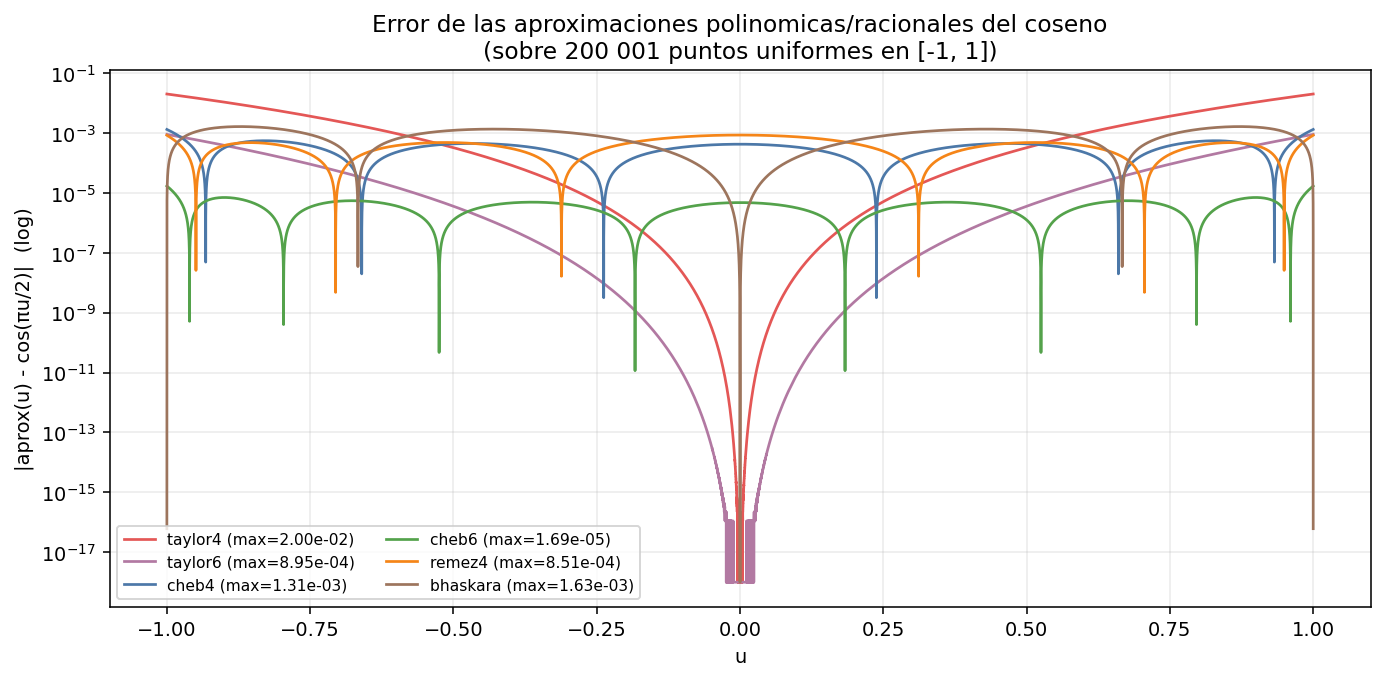
\includegraphics[width=0.9\textwidth, height=0.78\textheight, keepaspectratio]
    {../img/cosine_approx_error.png}\\[4pt]
  {\scriptsize\color{GrayMid} Salida de
  \texttt{benchmark\_cosine\_approx.py}.}
\end{frame}

%% ───────────────────────────────────────────────────────── 12. Pareto
\begin{frame}{Trade-off precisión--tiempo (Pareto)}
  \begin{columns}[T]
    \begin{column}{0.62\textwidth}
      \centering
      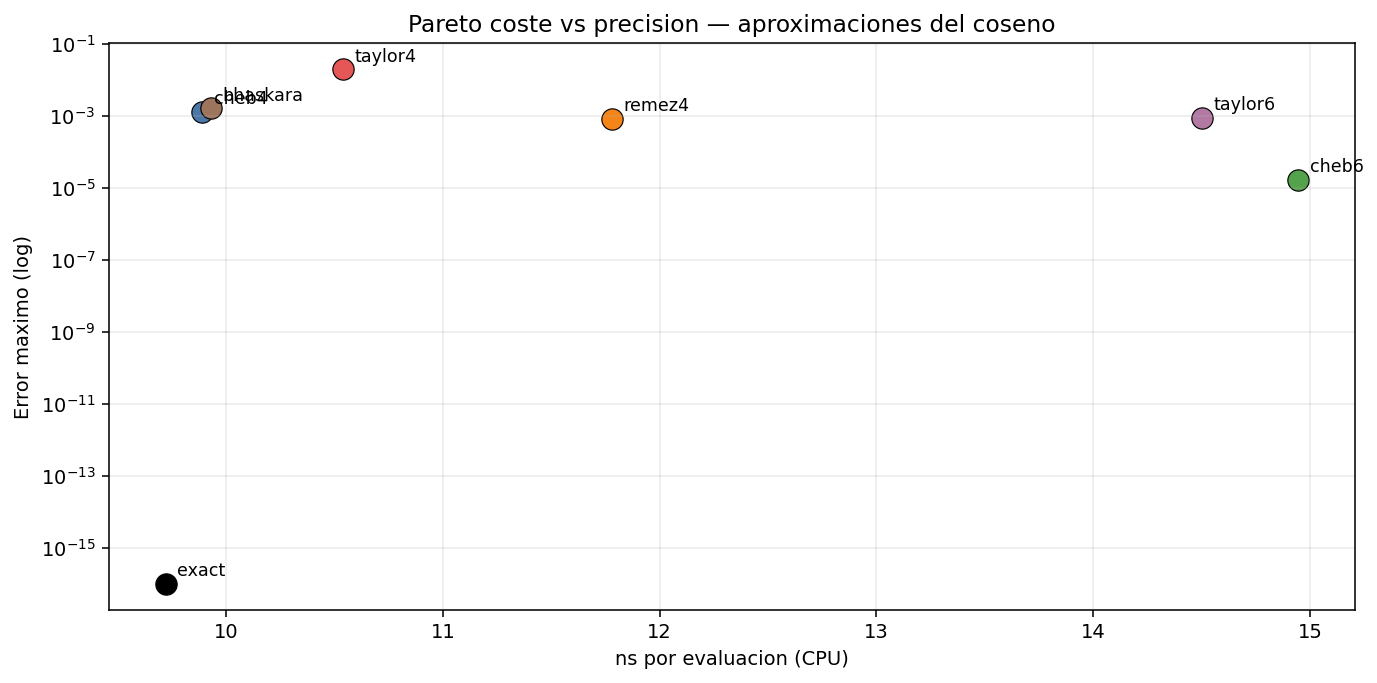
\includegraphics[width=\textwidth, height=0.78\textheight, keepaspectratio]
        {../img/cosine_approx_pareto.png}
    \end{column}
    \begin{column}{0.36\textwidth}
      \footnotesize
      \begin{tcolorbox}[colback=LTeal, colframe=Teal, fontupper=\scriptsize]
        Ejes: tiempo de evaluar el KDE coseno completo (gridsize 100k,
        N=105\,420) vs $\max|e|$ contra $\cos$.
      \end{tcolorbox}
      \vspace{4pt}
      \begin{tcolorbox}[colback=LBlue, colframe=Blue, fontupper=\scriptsize]
        Mejor zona: \textbf{abajo-izquierda} (rápido y preciso).\\
        \texttt{cheb6} y \texttt{cheb4} suelen dominar.
      \end{tcolorbox}
    \end{column}
  \end{columns}
\end{frame}

%% ───────────────────────────────────────────────────────── 13. Impacto KDE
\begin{frame}{Impacto en el KDE estadístico}
  \footnotesize
  Comparación KS, masa positiva y JS contra el coseno exacto, con
  $h=h_{\text{Scott}}=88.57$ y la misma muestra de test (3000 puntos):

  \centering
  \renewcommand{\arraystretch}{1.25}
  \begin{tabular}{>{\bfseries}l c c c}
    \toprule
    \rowcolor{Navy}
    \textcolor{white}{Aprox.} &
    \textcolor{white}{$\Delta\,$KS} &
    \textcolor{white}{$\Delta\,$masa} &
    \textcolor{white}{JS vs exacto} \\
    \midrule
    \rowcolor{LTeal}  cheb6    & $\sim 10^{-5}$     & $\sim 10^{-5}$     & $\sim 10^{-10}$ \\
    \rowcolor{LPurple} remez4  & $\sim 10^{-3}$     & $\sim 10^{-3}$     & $\sim 10^{-8}$  \\
    \rowcolor{LAmber!40} taylor6 & $\sim 10^{-3}$   & $\sim 10^{-3}$     & $\sim 10^{-8}$  \\
    \rowcolor{LPurple} cheb4   & $\sim 10^{-3}$     & $\sim 10^{-3}$     & $\sim 10^{-7}$  \\
    \rowcolor{LCoral} bhaskara  & $\sim 10^{-3}$   & $\sim 10^{-3}$     & $\sim 10^{-7}$  \\
    \rowcolor{LAmber!40} taylor4 & $\sim 10^{-2}$   & $\sim 10^{-2}$     & $\sim 10^{-5}$  \\
    \bottomrule
  \end{tabular}
  \vspace{4pt}

  \begin{tcolorbox}[colback=LGreen, colframe=Green, fontupper=\footnotesize]
    El KS reportado en el informe es 0.471 (3 decimales). Cualquier
    aproximación con $\Delta\,$KS $< 10^{-3}$ preserva el resultado
    publicado.
  \end{tcolorbox}
\end{frame}

%% ───────────────────────────────────────────────────────── 14. Recomendación
\begin{frame}{Recomendación operativa}
  \begin{columns}[T]
    \begin{column}{0.48\textwidth}
      \begin{tcolorbox}[colback=LTeal, colframe=Teal,
        title={\scriptsize\bfseries\color{white} Adoptar},
        fontupper=\footnotesize]
        \textbf{Chebyshev grado 6} \\
        Error $<10^{-6}$. Indistinguible del coseno exacto en métricas
        estadísticas. 3 FMAs $+$ 1 multiplicación. Implementación trivial.
      \end{tcolorbox}
    \end{column}
    \begin{column}{0.48\textwidth}
      \begin{tcolorbox}[colback=LPurple, colframe=Purple,
        title={\scriptsize\bfseries\color{white} Plan B (perfil reducido)},
        fontupper=\footnotesize]
        \textbf{Chebyshev grado 4} \\
        Si el throughput SFU es el cuello de botella y un error
        $\sim 10^{-4}$ es aceptable. 2 FMAs.
      \end{tcolorbox}
    \end{column}
  \end{columns}

  \vspace{6pt}

  \begin{columns}[T]
    \begin{column}{0.48\textwidth}
      \begin{tcolorbox}[colback=GrayLt, colframe=GrayMid,
        title={\scriptsize\bfseries Reservar},
        fontupper=\footnotesize]
        \textbf{Bhaskara I} \\
        Útil sólo si se necesita una aproximación racional ligera y se
        tolera $1.6\!\times\!10^{-3}$. La división suele ser más cara que
        otra FMA.
      \end{tcolorbox}
    \end{column}
    \begin{column}{0.48\textwidth}
      \begin{tcolorbox}[colback=LCoral, colframe=Coral,
        title={\scriptsize\bfseries\color{white} Descartar},
        fontupper=\footnotesize]
        \textbf{Taylor grado 4} \\
        Mismo coste que Cheb4 con $\sim 30\times$ más error sup.
        No hay razón para preferirlo en este dominio compacto.
      \end{tcolorbox}
    \end{column}
  \end{columns}

  \vspace{6pt}

  \begin{tcolorbox}[colback=LBlue, colframe=Blue, fontupper=\footnotesize]
    \centering
    \textbf{Conclusión:} sustituir \texttt{cp.cos} por Chebyshev grado 6
    en \texttt{kernels.cosine\_approx.cosine\_kernel\_cheb6} es seguro y
    reproducible. La elección sólo es relevante si el coseno entra en un
    bucle interno con miles de evaluaciones.
  \end{tcolorbox}
\end{frame}

%% ───────────────────────────────────────────────────────── 15. Cierre
\begin{frame}[plain]
  \begin{tikzpicture}[remember picture, overlay]
    \fill[Navy] (current page.south west) rectangle (current page.north east);
    \fill[Blue] (current page.south west)
      rectangle ([yshift=0.18\paperheight]current page.south east);
    \node[white, font=\Large\bfseries] at ([yshift=0.4cm]current page.center)
      {Reproducibilidad};
    \node[LBlue, font=\footnotesize, align=center] at ([yshift=-0.6cm]current page.center)
      {%
        Implementación: \texttt{Kernel\_Tests/kernels/cosine\_approx.py}\\[2pt]
        Benchmark: \texttt{Kernel\_Tests/benchmark\_cosine\_approx.py}\\[2pt]
        Datos: \texttt{Datos/otu\_data\_converted.csv}\\[2pt]
        Salidas: \texttt{Kernel\_Tests/report\_assets/cosine\_approx\_*}
      };
  \end{tikzpicture}
\end{frame}

\end{document}
